\documentclass[a4paper,12pt]{article}
\usepackage[utf8]{inputenc}
\usepackage[T1]{fontenc}
\usepackage[italian]{babel}
\usepackage[margin=2.5cm]{geometry}
\usepackage{amsmath}
\usepackage{graphicx}
\graphicspath{{immagini/}}
\usepackage[colorlinks=true,urlcolor=blue,linkcolor=black,citecolor=black]{hyperref}

\title{Studio sperimentale dell'algoritmo di Grover}
\author{} % Inserire nome e cognome.
\date{}

\begin{document}
\maketitle

\section{Introduzione}
In questo progetto studio l'algoritmo di Grover, che permette di cercare una
soluzione in uno spazio non strutturato mediante l'amplificazione delle
ampiezze. L'obiettivo degli esperimenti \`e capire come cambia la probabilit\`a
di successo al variare del numero di iterazioni e quanto il comportamento
ideale si discosta da quello osservato in presenza di rumore.

Il percorso parte dalla costruzione visuale dei circuiti con Quantum
Programming Studio e IBM Quantum Composer e prosegue con l'implementazione in Qiskit, le simulazioni e le
prove su hardware IBM. In questa prima parte mi concentro sul ruolo delle
porte e sui cambiamenti dello stato quantistico durante l'algoritmo.


\section{Primi esperimenti con strumenti visuali}
Per iniziare ho costruito due piccoli circuiti attraverso strumenti di
composizione visuale: il primo con Quantum Programming Studio\footnote{
Quantum Programming Studio, \url{https://quantum-circuit.com/docs/}.},
il secondo con IBM Quantum Composer\footnote{IBM Quantum Composer,
\url{https://quantum.cloud.ibm.com/docs/en/guides/composer}.}.
Ho inserito le porte direttamente sulle linee dei qubit, seguendo da sinistra
a destra le operazioni di preparazione, oracolo, diffusore e misura.
Questo approccio mi ha permesso di ragionare sulle singole operazioni prima
di passare alla costruzione dei circuiti in Python.

Entrambi gli esempi utilizzano due qubit di ricerca, quindi quattro stati
possibili. Le porte Hadamard iniziali preparano la sovrapposizione uniforme:
\[
 |s\rangle=\frac{|00\rangle+|01\rangle+|10\rangle+|11\rangle}{2}.
\]
Ogni stato ha inizialmente probabilit\`a $1/4$. L'oracolo cambia il segno
dell'ampiezza della soluzione; il diffusore trasforma questa differenza
di fase in amplificazione. Nei due circuiti ho usato una sola iterazione.
Per evitare ambiguit\`a, nel seguito scrivo gli stati nell'ordine $|q_1q_0\rangle$:
il qubit $q_0$, disegnato in alto, corrisponde al bit a destra.

\subsection{Quantum Programming Studio: circuito senza ancilla}
Nel primo circuito ho utilizzato soltanto i due qubit di ricerca.
L'oracolo \`e costruito con porte $X$, Hadamard e una CNOT.
Una Hadamard sul target prima e dopo la CNOT permette di ottenere
una porta controlled-$Z$:
\[
 (I\otimes H)\,\mathrm{CNOT}\,(I\otimes H)=\mathrm{CZ},
\]
intendendo qui il secondo fattore come il qubit target della CNOT.
La CZ cambia il segno dello stato in cui entrambi i qubit valgono uno.
Le due porte $X$ sul qubit $q_0$, poste prima e dopo questo blocco,
spostano la condizione al caso $q_0=0$, $q_1=1$.
La soluzione marcata \`e quindi $|10\rangle$ nella convenzione adottata.

Dopo l'oracolo, il diffusore applica $H$ e $X$ a entrambi i qubit,
poi una seconda CZ, ancora realizzata con H--CNOT--H sul target,
e infine annulla le $X$ e applica le Hadamard finali.
Il qubit target delle CNOT fa parte del registro di ricerca:
non viene aggiunto un qubit ausiliario.

\begin{figure}[htbp]
    \centering
    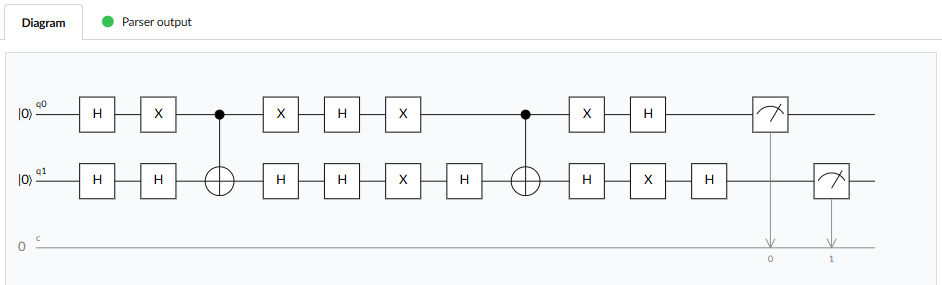
\includegraphics[width=\textwidth]{QPS.png}
    \caption{Circuito realizzato in Quantum Programming Studio con due
    qubit di ricerca, senza ancilla.}
    \label{fig:studio}
\end{figure}

\subsection{Quantum Composer: circuito con ancilla}
Nel secondo circuito ho mantenuto due qubit di ricerca e aggiunto
un terzo qubit, indicato con \texttt{anc[0]} nello screenshot.
Questo qubit non rappresenta un ulteriore bit della soluzione:
lo spazio di ricerca rimane di quattro stati.
Le porte $X$ e $H$ preparano l'ancilla nello stato
\[
 |-\rangle=\frac{|0\rangle-|1\rangle}{\sqrt{2}}.
\]
L'oracolo \`e una Toffoli con i due qubit di ricerca come controlli
e l'ancilla come target. Poich\'e $X|-\rangle=-|-\rangle$,
quando entrambi i controlli valgono uno si introduce un segno meno
nell'ampiezza corrispondente. Questo meccanismo si chiama
\emph{phase kickback}: l'ancilla permette di modificare la fase dello stato
$|11\rangle$, pur rimanendo nello stato $|-\rangle$.

Per costruire il diffusore applico $H$ e $X$ sui qubit di ricerca,
riutilizzo la Toffoli con la stessa ancilla, quindi applico nuovamente
$X$ e $H$. Alla fine misuro soltanto i due qubit di ricerca.
In Figura~\ref{fig:composer}, l'ancilla \`e la linea \texttt{anc[0]}.

\begin{figure}[htbp]
    \centering
    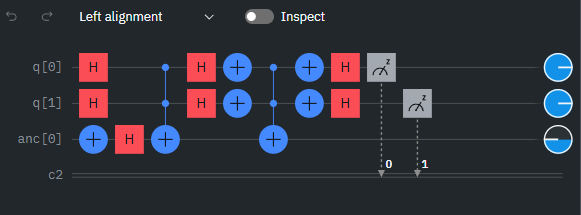
\includegraphics[width=\textwidth]{IBMComposer.png}
    \caption{Circuito realizzato in IBM Quantum Composer:
    due qubit di ricerca e un'ancilla per il phase kickback.}
    \label{fig:composer}
\end{figure}

\subsection{Confronto e funzionamento dei due circuiti}
Le due costruzioni realizzano la stessa idea di Grover con risorse diverse.
Il primo circuito modifica direttamente le fasi del registro attraverso
una CZ decomposta; il secondo ottiene la modifica di fase usando un'ancilla.
Questa differenza dipende dalla costruzione scelta, non da un obbligo
imposto dai due strumenti grafici. Inoltre i target sono diversi:
$|10\rangle$ nel primo circuito e $|11\rangle$ nel secondo.

Dopo l'oracolo l'ampiezza della soluzione vale $-1/2$ e le altre valgono
$1/2$. La loro media \`e $1/4$: il diffusore standard trasforma
ogni ampiezza $a$ in $2\bar a-a$, portando quella della soluzione a 1
e le altre a 0. Le sequenze mostrate realizzano il diffusore a meno
di un segno globale, che non modifica le probabilit\`a di misura.

Ho verificato le sequenze ricostruite con una simulazione ideale Statevector:
il primo circuito restituisce $q_0=0$, $q_1=1$, mentre il secondo restituisce
$q_0=q_1=1$, entrambi con probabilit\`a numericamente pari a 1.
Si tratta di una verifica dei circuiti delle immagini, non di conteggi
sperimentali raccolti dai due strumenti o di risultati hardware.

Questi primi esempi mostrano quindi che l'ancilla non \`e indispensabile
per costruire Grover: \`e un modo alternativo di realizzare l'oracolo e
il diffusore. In entrambi i casi l'oracolo da solo cambia le fasi,
mentre l'amplificazione delle probabilit\`a compare dopo il diffusore.

\end{document}
